\documentclass[
  utf8,%     More capable input encoding than latin-1.
  % parskip,%  For vertical whitespace between paragraphs.  This comes down to more than just using parskip.sty, so it's better to use this class option.
  % S5MP % If you intend to really use margin paragraphs (not recommended!).
%  crop,%     Produce output with crop marks and paper size A4.  Liu-Tryck should like this.  Automatically adds information, including the physical page number, at the top of each page.
       %     Add option 'noInfo' to suppress the info at the top of each page when using option 'crop'.
  % Font options: 'kp' (default), 'times', 'lm'.  The KpFonts (loaded using 'kp'), is the most complete font among the provided options.  Among other, it supports slanted small caps.  See rtthesis.cls for more details regarding the font options.
  largesmallcaps,intlimits,widermath,% Good options to KpFonts.
  sharecounter,nobreak,definition=marks,%  See comments in the results chapter of this document for more information on these options!
  %numbers, % If you want to cite references by numbers, use this option.
  noparts% Use option 'noparts' if you do not make use of part divisions.
]{rtthesis}
\usepackage[T1]{fontenc}
\usepackage[bitstream-charter]{mathdesign}
\usepackage[font=footnotesize,labelfont=bf]{caption}
%\usepackage{listings}
%\usepackage[parfill]{parskip}
%\usepackage{float}
%\usepackage{graphicx}
%\usepackage[swedish]{babel}
%\usepackage[applemac]{inputenc}
\usepackage{mythesis}




\begin{document}
\selectlanguage{english}
\makeFrontPage
\frontmatter
\maketitle
\makeLibraryPage{The properties of free-standing cubic silicon carbide for optoelectronic applications are explored in this work. The main focus of the work is on boron doped cubic silicon carbide, which is proposed as a highly useful material in several optoelectronic applications. The material is grown using sublimation epitaxy and the doped material is grown homoepitaxially on nominally undoped seeds. It is characterized using the experimental setups of photoluminescence spectroscopy, Nomarski interference spectroscopy and absorption spectroscopy. 

I study seed growth of nominally undoped cubic material on hexagonal (4H) substrates, and the influence on the grown material from the different faces of the substrate. It is found that it is not possible under the explored conditions to completely cover the growth area with the cubic polytype on the carbon face, but it can be done reproducibly on the silicon face. Reasons for this are discussed. Different doping setups are also explored.

The influence on the material properties from growth conditions is explored. It is shown from absorption measurements that it is possible to grow boron doped cubic silicon carbide using this growth method, but optical microscopy studies show that the sample quality degrades with high doping concentrations. 

I explore the luminescence properties of the material. No boron related emission is found with either room temperature or low temperature photoluminescence spectroscopy. Reasons for this are discussed using results from absorption measurements and optical microscopy. 

}

\begin{abstract}[english]
  The properties of free-standing cubic silicon carbide for optoelectronic applications are explored in this work. The main focus of the work is on boron doped cubic silicon carbide, which is proposed as a highly useful material in several optoelectronic applications. The material is grown using sublimation epitaxy and the doped material is grown homoepitaxially on nominally undoped seeds. It is characterized using the experimental setups of photoluminescence spectroscopy, Nomarski interference spectroscopy and absorption spectroscopy. 

I study seed growth of nominally undoped cubic material on hexagonal (4H) substrates, and the influence on the grown material from the different faces of the substrate. It is found that it is not possible under the explored conditions to completely cover the growth area with the cubic polytype on the carbon face, but it can be done reproducibly on the silicon face. Reasons for this are discussed. Different doping setups are also explored.

The influence on the material properties from growth conditions is explored. It is shown from absorption measurements that it is possible to grow boron doped cubic silicon carbide using this growth method, but optical microscopy studies show that the sample quality degrades with high doping concentrations. 

I explore the luminescence properties of the material. No boron related emission is found with either room temperature or low temperature photoluminescence spectroscopy. Reasons for this are discussed using results from absorption measurements and optical microscopy. 


\end{abstract}
\begin{acknowledgments}
  Acknowledgements are pointless. Everyone was terrific, good on you!

  \addvspace{1em}
  \begin{flushright}
    \textit{%
      Linköping, Januari 2015\\
      Mattias Jansson%
    }
  \end{flushright}
\end{acknowledgments}

\tableofcontents
%\include{notation}

\mainmatter

%-*- mode: LaTeX; -*-

\chapter{Introduction}
%This thesis deals with SiC 
%Good properties when it comes to stability
%Used in power electronics, radiation (space - Citation needed!)

%SiC is a semiconductor
%Exists in a number of different polytypes
% This thesis deals with the cubic polytype
%One of the most common polytypes

% Difficulty in fabricating 3C with good quality
% Using sublimation epitaxy (FSGP)

% The band gap of 3C is good for solar cell applications
% And for water splitting
% Using doping to enhance the properties

% This thesis deals with examination of optical properties 
% List the characterization methods

% Describe the chapters

This thesis describes the growth and optical characterization of cubic silicon carbide (\emph{SiC}). SiC is a semiconductor which has attracted academic interest since the 19:th century, when it was first fabricated and used as an abrasive \cite{Acheson1893}. SiC has been found to be a very stable material. It exhibits a high chemical inertness \cite{Hume1941}, and is currently commonly used in high power and high temperature applications due to its ability to survive in such environments [Citation?]. 

SiC is a material which exists in a large number of different polytypes, the most common of which are hexagonal, cubic and rhombohedral. The work described in this thesis deals with the only cubic polytype, denoted \emph{3C}. This is one of the structurally most simple polytypes. Compared to the hexagonal counterparts 4H and 6H, the 3C polytype has for a long time been difficult to fabricate in good quality single crystal form, and is therefore less studied than the hexagonal types [Citation needed]. Recently a method of fabricating good quality material has been reported, using sublimation epitaxy \cite{Jokubavicius2014}. The method, called fast sublimation growth process (\emph{FSGP}), has been used to grow the samples used in the work described in this thesis. %Should decide how I should call 3C (3C-SiC, cubic SiC...?)

Cubic SiC has many interesting material properties, which have given rise to several proposals of applications for 3C. Some of these proposed applications are not possible to create with the hexagonal polytypes, but are unique for the cubic polytype. One such application is the use of boron doped 3C in an impurity photovoltaic solar cell (\emph{IPV}). This is suitable for 3C due to its band gap size together with the binding energy of boron as an acceptor in the material, which is almost ideal for photovoltaic cell material. This would give a significant increase in photovoltaic cell efficiency compared to the currently commercially available alternatives \cite{Richards2003}[Current efficiencies citation needed]. Another proposed application of 3C is as a photo-electrode in a photoelectrochemical cell used for water splitting \cite{Kato2014,Yasuda2012}, where solar energy is used in the decomposition of water into hydrogen and oxygen gas. 

This thesis deals with characterization of the optical properties of boron doped 3C-SiC. This is done using absorption spectroscopy, photoluminescence spectroscopy, \dots. Chapter \ref{sec:sic} gives an introduction to silicon carbide, its structure and properties. Chapter \ref{sec:growth} describes the process of growing the material. Both growth of undoped and boron doped material is described here. In chapter \ref{sec:characterization} a description of the different characterization methods is given, together with a theoretical description of what the measurements can tell about material properties. Chapter \ref{sec:experimental} describes how the experiments were done and chapter \ref{sec:results} describes the results obtained from the experiments. The results are discussed in chapter \ref{sec:discussion}. Chapters \ref{sec:conclusion} and \ref{sec:future} discuss what has been learned about the material and how the work should be continued in the future. 




































\label{sec:introduction}

%-*- mode: LaTeX; -*-

%Consists of Si and C atoms, crystal. (Arranged periodically)
%There exists many (Citation?) different kinds of polytypes
%Polytypes can be thought of as stacking sequence of hexagonal layers
%Base is one C and one Si
%Si and C faces, what is that? [Do I need this?]
%If I do anything on bulk, then I should discuss planes here. (Since the goal is to have (100) plane).

%The atoms are bonded together by covalent bonds.
%The band structure is shown...
%Indirect band gap of...
%Phonons

%Some relevant properties
%Mobility
%Dielectric constant

%Nitrogen as background doping
%Possible acceptors are
%Boron doping gives good band diagram as seen...


\chapter{An introduction to silicon carbide}
\label{sec:sic}
This chapter describes the properties of SiC which are relevant to this thesis. Section \ref{sec:crystal_structure} describes the atomic arrangement in the material, and some different arrangements are discussed. Section \ref{sec:band_structure} discusses the energy band structure of 3C-SiC. Finally section \ref{sec:doping_in_3C} describes how doping is achieved in a material and some of its effects in 3C-SiC. 

\section{Crystal structure}
\label{sec:crystal_structure}
Silicon carbide is a crystalline material consisting of silicon and carbon atoms. The crystalline nature of the material means that the atoms are arranged in a periodically repeating structure called a \emph{lattice}. For given chemical elements there may be several different ways to arrange the atoms in a lattice, i.e. different chemical compounds of the same atomic species. This is called \emph{polytypism}, where the different lattice structures are called the \emph{polytypes} of the material. Silicon carbide has a large number of different polytypes - there are more than 250 known polytypes of SiC \cite{Cheung2006}. The different polytypes can be described as different stacking orders of layers of atoms \cite{Mirgorodsky1995}. Figure \ref{fig:hex} shows one such layer. The depicted layer is the (111) surface. Each circle symbolizes one carbon and one silicon atom, displaced a small distance from each other. This pair of atoms is called the \emph{base} of the crystal. 

\begin{figure}[h]
\begin{center}
\includegraphics[scale=1]{lattice2.pdf}
\caption{Atomic arrangement of the atoms in each (111) layer. Here each sphere corresponds to one carbon and one silicon atom, as shown by the arrow. 
\label{fig:hex}}
\end{center}
\end{figure}

The marked hexagon in figure \ref{fig:hex} marks an area of the crystal plane which can be used to define the different polytypes, where the polytypes are defined by the placement of the base atoms in this area in different layers. Figure \ref{fig:poly} shows these stacking sequences for three of the most common polytypes. The depicted orders of the layers refer to one period in the periodic structure. The names for the different polytypes are stated at the top of the figure. The digit in the name refers to the number of layers of a period and the letter denotes the crystal symmetry. The letter \emph{H} denotes the hexagonal polytypes, whereas \emph{C} stands for the cubic polytype. Another common polytype is the 6H-SiC, which thus is a hexagonal structure with a period of six base layers. It should be noted that the 2H-SiC structure is the wurtzite structure and the 3C-SiC is the zincblende structure. The unit cell of the zincblende, or 3C-SiC, crystal has a lattice constant of $\mathrm{a} = 4.35$ Å \cite{Bimberg1981}. 


%\begin{figure}[h]
%\begin{center}
%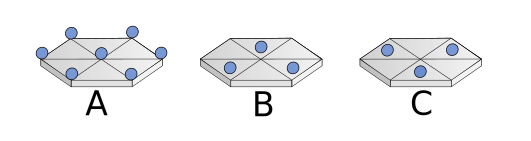
\includegraphics[scale=0.7]{hex5.pdf}
%\caption{Different atomic placements for the layers
%\label{fig:stacking1}}
%\end{center}
%\end{figure}


\begin{figure}[h]
\begin{center}
\includegraphics[scale=0.8]{poly.pdf}
\caption{Stacking order for the three most simple polytypes. 
\label{fig:poly}}
\end{center}
\end{figure}

\section{Band structure}
\label{sec:band_structure}
%The atoms are bonded together by covalent bonds.
%The band structure is shown...
%Energy gap - no available energy states
%valence and conduction bands
% Indirect band gap value
	%Change of k, momentum
%Direct band gap value. 

In SiC the atoms are bonded together with covalent bonds into a crystal. When the atoms are bonded together, the energy levels for the electrons in the material are defined by the material and lattice structure. This means that all materials have characteristic energy levels. When many atoms are bound together in a periodically repeating manner, as is the case in crystals, the discrete energy levels for the electrons in the atoms merge together to form continuous bands which are called energy bands. 

The band structure for 3C-SiC is shown as a band diagram in figure \ref{fig:band}. In this figure, each curve describes allowed energies for the electrons, and the spaces in between the curves are not allowed. The x-axis shows different points in reciprocal space, or \emph{k-space}. The marked points are specific points in the first brillouin zone of k-space, and the intermediate intervals form straight lines between the points. This figure has been obtained using the approximate method of pseudopotentials, as described in \cite{Aourag1994}. The zero point energy has been chosen to be at the $\Gamma$-point in k-space. 

The grayed area in the figure is the \emph{band gap} of the material, since there are no allowed electronic states in this area. The band below the band gap is called the valence band, and the band above is called the conduction band. For 3C-SiC, as is characteristic for semiconductors, the Fermi level is in the middle of the band gap. This means that at the temperature of 0 K all electrons will be in the valence band, and the conduction band will be unoccupied. When the conduction band is unoccupied the material will not be able to conduct electricity. If the temperature is raised above 0 K there will be some occupation of the conduction band and some electrical conduction will be possible. With a higher temperature there will be more electrons in the conduction band and thus a higher conductivity of the material. One way to change the position of the Fermi level is to introduce impurities into the crystal, i.e. doping. This will be discussed later. 

\begin{figure}[h]
\begin{center}
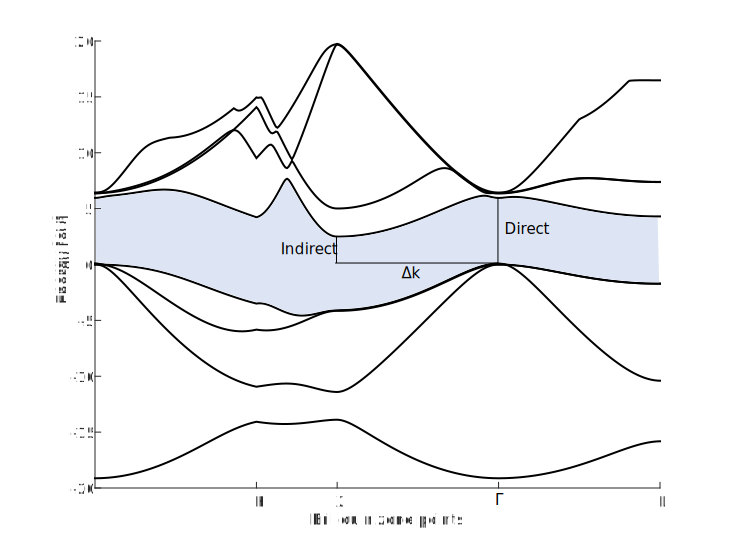
\includegraphics[scale=0.6]{band_diagram2.pdf}
\caption{The band diagram of SiC at ambient conditions for different positions in the Brillouin zone. The indirect and direct band gaps are marked in the figure. The marked area is the band gap. The energy levels have been obtained using the pseudopotential method, as described in \cite{Aourag1994}.
\label{fig:band}}
\end{center}
\end{figure}

In the figure \ref{fig:band} it can be seen that the smallest energy difference between the valence and conduction bands is between the $\Gamma$-point in the valence band and the X-point in the conduction band. This difference is called the \emph{band gap energy}. The difference between the $\Gamma$- and X-points is called the indirect band gap, while the difference between the values at the $\Gamma$-point is called the direct band gap, as illustrated in the figure. These values are given in table \ref{tab:eg}. The value for the room temperature band gaps are taken from the simulation, whereas the 2 K value is taken from literature. 

\begin{table}[h]
\caption{Values for the indirect and direct band gap energies. The indirect values are given both for room temperature and low temperature, as this will be of value later in the thesis.}
\label{tab:eg}
\begin{center}
\begin{tabular}{ l c r }
  \hline                       
  \hline       
  \vspace{1mm}
    $\mathrm{E_{g,indirect}}$  (300 K) & $\mathrm{E_{g,indirect}}$ (2 K) & $\mathrm{E_{g,direct}}$  (300 K)\\
    \hline
  2.36 eV & 2.42 eV \cite{Bimberg1981} & 6.00 eV\\
  \hline  
\end{tabular}
\end{center}
\end{table}

When an electron makes the indirect transition from the valence to the conduction band the energy is increased by E$_\mathrm{g,indirect}$, and the k-value is changed, as indicated by $\Delta \mathrm{k}$ in figure \ref{fig:band}. This change of k-value implies a change in momentum of the electron, since k and momentum p is related by
\[p = \hbar k,\]
where $\hbar$ is Dirac's constant. This is of importance when studying interaction between the material and light. Photons are capable of providing the energy needed to transit from the valence to the conduction band, but cannot provide the change of momentum needed. The law of conservation of momentum requires the total momentum of the system to be preserved during the transitions. The extra momentum can come from interaction with \emph{phonons}, which are vibrations in the crytsal. 

The phonon energy spectrum has four ground modes since there are two different kinds of atoms in the material. There are the acoustic and optical phonon modes. Theoretical calculations of the phonon dispersion curves for 3C-SiC have been done by Karch et al. \cite{Karch1994}. They show the four modes: TA, LA, TO, LO, and give the wavelength for each mode. The transition in k-space for the indirect transition is between the $\Gamma$- and the X-points, hence it is of interest to know which phonon wavelengths and energies this corresponds to.  Table \ref{tab:phonons} shows these computed wavelengths and the corresponding energies, which have been calculated using the fact that

\[E_\mathrm{meV} = \frac{hc(\frac{1}{\lambda_{\mathrm{cm}}})}{e}\times 10^5,\]

\noindent where h is Planck's constant, c is the speed of light and e is the elementary charge. 

\begin{table}[h]
\caption{Inverted wavelengths and energies for the $\Gamma$-X tranistion. Values for $\lambda$ from \cite{Karch1994}.}
\label{tab:phonons}
\begin{center}
\begin{tabular}{ l l l }
  \hline                       
  \hline       
  \vspace{1mm}
    Mode  & $\lambda^{-1} [\mathrm{cm}^{-1}]$  & E [meV]\\
    \hline
  TA &  368 & 45.6\\
  LA &  637 & 79.0\\
  TO &  760 & 94.3\\
  LO &  829 & 102.9\\
  \hline  
\end{tabular}
\end{center}
\end{table}





%\section{Some properties}
%\label{sec:}




\section{Doping in 3C-SiC}
\label{sec:doping_in_3C}

% Doping is when an atom is replaced
% Donors and acceptors, number of valence electrons. 
% Donors can donate, acceptors accept, as seen in fig. 
	% Nitrogen doping, more electrons
	% Ionization energy 
	% Difficult to avoid
	
	% Some possible acceptors
	% And their energies
	% Refer to section about B-doped solar cells. 
% Doping can be achieved...
% Problems which can occur with doping are...


Doping is a way to change the electronic structure of a material by substituting some of the native atoms with a foreign element. In the case of SiC this means that either silicon or carbon is replaced by some other element. The band structure of the material changes depending on which impurity is introduced to the crystal. By choosing the dopants it is possible to tailor the band structure to create various new properties of the material. 

An important factor for how the band structure is changed is the number of valence electrons in the introduced element, compared to the element it replaces. Silicon and carbon both have four valence electrons, creating four bonds to its neighbouring atoms in the crystal. The electrons are strongly bound to the atomic nuclei, requiring energy corresponding to the band gap to free one electron. If one silicon or one carbon atom is replaced by an element with five valence electrons, the additional electron is not as strongly bound to the nucleus and can easily release an electron to the conduction band. This is called a \emph{donor} atom. Similarly if an atom with only three valence electrons is introduced to the crystal, it can readily bind an electron from the valence band, creating an electron deficiency, or \emph{hole} in the valence band. This is called an \emph{acceptor} atom. Figure \ref{fig:dopant_band} shows a simplified band diagram with a donor and an acceptor level. The donor level donates an electron to the conduction band when the electron is supplied with the energy $\mathrm{E_D}$. The acceptor accepts an electron from the valence band when the electron is supplied with the energy $\mathrm{E_A}$. The energy required to supply the material with one carrier from a dopant level is called the \emph{binding energy} (or \emph{ionization energy}) of the dopant. 

\begin{figure}[h]
\begin{center}
\includegraphics[scale=0.6]{doped_band1.pdf}
\caption{Two new energy levels are introduced by doping. 
\label{fig:dopant_band}}
\end{center}
\end{figure}

As dopants are introduced in the material, the position of the Fermi level relative to the bands changes. The Fermi level resides in the middle of the band for undoped materials, but will move nearer to the conduction (valence) band as donors (acceptors) are introduced. This change in Fermi energy corresponds to a change in occupancy in the different levels. 

\subsection{Donors}
% What does it replace, Si or C?
Since silicon and carbon both have four valence electrons, a donor atom in SiC must have five or more electrons. One common donor is nitrogen, which has five valence electrons. The nitrogen atoms take the place of the carbon atoms in the lattice. This means that each added N-atom can supply the conduction band with one electron. A material with more electron carriers than the hole counterpart is said to be an \emph{n-type} material. Freitas et al. have measured the binding energy of nitrogen in 3C-SiC, and found it to be 54 meV \cite{Freitas1988}. This means that the lowest N-level is 54 meV below the conduction band.

Nitrogen doping can be achieved intentionally by fabricating the material in a nitrogen atmosphere, but nitrogen is always present in sublimation grown material even at vacuum conditions \cite{Sun2012b}. This means that material grown by this method is generally n-type, if no other impurity is present. The n-type material can also be created by other elements in group five.  Another possible donor in 3C-SiC is phosphorus, which has a binding energy of 48 meV \cite{Ivanov2010}. Reports of doping with As, P and Sb exist, but are far less common than N-doping \cite{Rao1999}. 

\subsection{Acceptors}
% What do they replace, Si or C?
Acceptor atoms need to have fewer valence electrons than silicon and carbon, which is why group three elements are the most common acceptors. Examples of acceptor materials are boron and aluminium, which have the binding energies 257 meV \cite{Freitas1988} and 735 meV \cite{Richards2003} respectively. A material with more hole carriers than the electron counterpart is said to be \emph{p-type}. Table \ref{tab:dopants} summarizes the different dopant energy levels. 

\begin{table}[h]
\caption{Binding energies for some of the most common SiC dopants.}
\label{tab:dopants}
\begin{center}
\begin{tabular}{ l l l r}
  \hline                       
  \hline       
  \vspace{1mm}
    Element  & Dopant type & E$_{D/A}$ [meV] & Reference\\
    \hline
  N &  Donor & 54 & \cite{Freitas1988}\\
  B &  Acceptor & 735 & \cite{Richards2003}\\
  Al &  Acceptor & 257  & \cite{Freitas1988}\\
  \hline  
\end{tabular}
\end{center}
\end{table}

The B-doping energy level is of particular interest for photovoltaic applications, where the binding energy is ideal for an application called \emph{intermediate band photovoltaic solar cell}. In this application, the electrons can make two different energy transitions. One transition can be done between the valence band and the impurity level, and one between the impurity  level and the conduction band. It has been shown that the binding energy of the B-acceptor in 3C-SiC is very well matched to the solar spectrum. Much of the emitted solar energy can be captured by the B-doped 3C-SiC \cite{Richards2003,Luque1997}. 
%This is described in more detail in chapter \ref{sec:intermediate_band_pvc}. 
\\ 

\noindent 
There are several ways to create doped materials. It can be done by ion implantation, where ions are accelerated to high energies and then made to collide with the undoped material \cite{Rao1999}. It can also be done as the material is grown, by including the doping element in the ambient. The first method has several advantages: it can be done with good control over doping density and it is possible to select only certain areas of the material to dope. The latter method is done \emph{in situ}, so it requires no additional equipment. It is also not as prone to create defects as the ion implantation method is, where annealing is often required after implantation in order to reduce the number of defects. In the work described in this thesis, the method of doping is to include the doping material during the growth. This method is described in more detail in chapter \ref{sec:growth}. 

During doping some of the native atoms are replaced. This will have effects on the quality of the produced material. Different elements have different atomic radii, so replacing one atom by one of a different element will create some strain in the material. This may lead to defects in the material. 





































\label{sec:sic}

\chapter{Growth technique}
\label{sec:growth}

% Description of various techniques. 
% FSGP
	% Uses sublimation
	% Different polytypes at different pressures
	% Setup
		% Describe the figure
	% Substrate
		% Off axis (compare on-axis) 
		% Cleaned
% Parameter space
	% Describe from book
	% Review of what has been done in group
% Growth of doped material. 

SiC can be fabricated by several different techniques, and the different techniques are advantageous for different polytypes and applications. Some of the most common methods are \emph{sublimation epitaxy}, \emph{liquid phase epitaxy (LPE)}, \emph{chemical vapour deposition (CVD)} and \emph{physical vapour deposition (PVD)} \cite{Ivanov1999}. 

The goal when growing freestanding material is to have high quality material of large volume. Up to this point in time, researchers have had more success fabricating high quality 4H and 6H material compared to 3C \cite{J.B.CASADYandR.W.JOHNSON1996}. The hexagonal polytypes are commonly fabricated using PVD. This method has not been widely adapted to 3C growth however, which is often attributed to the fact that this method uses homoepitaxy, and there are no 3C seeds widely available. Historically in the growth of 3C using CVD, there has been a trade-off between crystal quality and growth rate. Nishino et al. reported in 1983 a growth rate of approximately 2.5 microns per hour with the CVD technique for 3C growth \cite{Nishino1983}. This rate is much too low to create free standing material. The growth rate for CVD growth has been improved since this time, and in 2002 Nagasawa et al. reported a rate of 40 $\mu$m/h \cite{Nagasawa2002}, which makes it possible to fabricate free standing 3C. 

Another growth method is sublimation epitaxy, which was demonstrated by Lely in 1955 \cite{Lely1955}. In this method material is transferred between a source material and a substrate using the fact that SiC sublimes. Recently there have been reports of high quality cubic SiC fabricated by a type of sublimation epitaxy called \emph{fast sublimation epitaxy (FSGP)}. Growth rates as high as 500 $\mu$m/h have been reported using this method, while still having good quality material \cite{Jokubavicius2014}. This high growth rate is obviously ideal for growth of free standing (and even bulk) material. This chapter describes in detail the sublimation method in general and FSGP in particular. FSGP is the method used to obtain the results in this thesis. 
 
 \section{About sublimation and nucleation}
 % What is sublimation, how does it work?
 % What governs the process?
 Sublimation is the phase transition where a material transitions between solid and gas, without the intermediate liquid phase. At normal conditions SiC does not melt, but rather it sublimes. For SiC to melt a pressure of 100,000 atm and a temperature of at least 3200 $^\circ$C is required. At atmospheric pressure SiC can only sublime \cite{Scheel2003}. Sublimation of a SiC source material will give a vapour consisting of different molecules consisting of silicon and carbon, for example $\mathrm{Si, Si_2C, SiC_2}$ etc. The composition and vapour pressure of the gas can be controlled using parameters such as temperature and pressure of the ambient. 
 
If a substrate is placed in the silicon-carbon vapour some of the material will be adsorbed on the surface of the substrate, in the form of \emph{adatoms}. When many such atoms are adsorbed at the surface they bind together, forming a \emph{nucleus} of crystal growth. In a sublimation growth setup, a source of SiC is heated, initiating the sublimation. The vapour then travels to an appropriate substrate, by the means of a heat gradient. Material is adsorbed on the substrate which forms the grown crystal. Figure \ref{fig:sublimation} shows a schematic of this process. 

\begin{figure}[h]
\begin{center}
\includegraphics[scale=1]{sublimation.pdf}
\caption{A vapour containing silicon and carbon molecules is created by sublimation of a SiC source. The vapour is adsorbed at the substrate. 
\label{fig:sublimation}}
\end{center}
\end{figure}
 
 As the material is adsorbed at the substrate the growth begins. The crystal growth is governed by the free energy of the whole system. A decrease in free energy works to promote the growth. In crystal growth, a decrease in free energy is also a decrease in chemical potential $\mu$, meaning that crystal growth is driven by a decrease in chemical potential. The system is made up by the vapour and the crystal phases. Hence a change in chemical potential is given by 
 \[\Delta \mu = \mu_v -\mu_c,\]
where $\mu_v$ is the chemical potential for the vapour and $\mu_c$ is for the crystal. For growth from vapour phase, the chemical potential difference between vapour and crystal is dependent on the \emph{vapour pressure} and the \emph{saturated vapour pressure} through the formula
 \[\Delta \mu = k_BT\log(p/p_e),\]
where p is the vapour pressure and p$_e$ is the saturated counterpart. Defining the \emph{supersaturation}, $\sigma$, as
\[\sigma = \frac{p-p_e}{p_e}\]
thus
 \[\Delta \mu = k_BT\log(\sigma+1).\]
Taking the first order Taylor expansion around $\sigma = 1$ this becomes
\[\Delta \mu \approx k_BT\sigma.\]
 It is concluded that the change in chemical potential is directly proportional to the supersaturation of the system. A decrease in supersaturation will hence promote growth and, as shown below, increase growth rate. 
 
 Growth of the crystal can occur in several ways. One such way is called \emph{lateral enlargement} or simply \emph{lateral growth}. This growth mode is present on smooth surfaces. For growth to occur there must exist a place where the adatoms can bind to the surface. One such place is at a step on the surface. Steps on the surface will contain \emph{kinks}, which can be described as corners in the step. An adsorbed adatom diffuses on the surface until it encounters such a step kink, where it attaches. As atoms are bound to the step, it moves forward with a certain velocity. This velocity can be shown \cite{Scheel2003} to be
\[v_{\infty} = \frac{2\lambda_s}{n_0}\frac{p_e}{\sqrt{2\pi mk_BT}}\sigma.\]

Here $\lambda_s$ is the diffusion length of an adatom before it gets desorbed from the surface. Moreover $n_0$ is the density of lattice points on the surface and m is the atom mass. It is important to note that the step velocity, and hence the growth rate, is linearly proportional to the supersaturation. 
 
 
% \section{Growth using FSGP}

 


 
 
 
 
 
 
 
 
 
 
 
 
 
 
 
 
 
 
 
 
 
 
 
 
 
 
 
 
 
 
 
 
 
 
 
 
 
 
 
 
 
 
 
\label{sec:growth}

%-*- mode: LaTeX; -*-

%Introduction to characterization
	%Optical properties and morphology
	%Electrical properties are also of interest, but beyond scope
%Absorption
	%General about absorption and transmission of semiconductors
	%Describe setup in general
	%How to compute coefficient and band edge
%PL measurements
	%General about excitation and recombination, luminescence 
		%How to infer the band structure from the PL-spectrum
	%
\chapter{Characterization techniques}
This chapter will describe the different characterization techniques. 

This is a paragraph.
\label{sec:characterization}
	%\subsection{Nomarski microscopy}
	%\subsection{Photoluminescence spectroscopy}
	%-*- mode: LaTeX; -*-

\section{Absorption measurements}
Here will follow a description of how the absorption measurements were done. 
	\label{sec:absorption}
	%\subsection{Hydrogen generation measurements}
	
%-*- mode: LaTeX; -*-

\chapter{Experimental setup}
Here the setups for the various experiments will be described. 
\label{sec:experimental}

%-*- mode: LaTeX; -*-

\chapter{Results}
This chapter describes the results obtained from the experiments. 
\label{sec:results}

%-*- mode: LaTeX; -*-

\chapter{Discussion}
\label{sec:discussion}
This chapter discusses the results presented in chapter \ref{sec:results}. The chapter is divided into two parts, one part discusses the results of seed growth and the other part discusses the results from characterization of the B-doped samples. 

\section{On seed growth}
As shown in section \ref{sec:results:seeds}, the carbon face grown seeds did not have complete coverage of cubic SiC on the terrace, yet the silicon face grown seeds could reproducibly be grown with complete cubic coverage. As seen in figure \ref{fig:supersaturation}, 2D growth is promoted by high supersaturation. A possible explanation of the results is that the supersaturation for the C-face growth was too low. The examined temperatures, as shown in table \ref{tab:seeds}  range from 1825 to 1925 $^\circ$C, which is a large portion of the parameter space in which the 3C-SiC polytype is stable. Changing the temperature much more during growth is unlikely to result in better 3C-coverage, since this will likely be outside the region where 3C-SiC can be formed in a stable manner. Because of this, the supersaturation will not be able to be changed much more by altering the temperature. 

From table \ref{tab:seeds} it can be seen that the percentage of the terrace covered by 3C-SiC does not show any trend with regards to temperature. The growth time has been adjusted to get similar sample thickness for all samples. In this way it was possible to vary only the supersaturation between samples. This indicates that for the used growth setup it is not possible to change the supersaturation enough to get complete 3C-SiC coverage of the terrace. It should however be mentioned that the pressure conditions for growth have not been explored in this work, and that it may be possible to alter the ambient pressure to get more cubic coverage. 

A possible explanation of the difference in 3C-SiC coverage on silicon and carbon face substrates is the spiral growth character. On Si-face the spirals take the form of proper spirals, with steps expanding from the spiral arms. The C-face spiral takes the form of straight lines extending radially from the center, as seen in figure \ref{fig:carbon_seed1}. The 3C-SiC polytype nucleates on top of the heteroepitaxially grown spirals and grows over the spiral steps. The spiral shape can then be expected to influence how the 3C-SiC is grown. The silicon face spiral may be advantageous for cubic growth, while the carbon face spiral may not be. Another possible explanation is that there may be some difference between how the Si- and C-surfaces look for off-axis cut samples. There may be a difference in the number and density of the steps, which in turn will influence the terrace growth. To get a proper understanding of this, electron microscopy would have to be done on the substrate surface and the terrace after initial nucleation. In this way a proper understanding of the growth mechanisms governing C- and Si-face growth would be possible. This is however beyond the scope of this work. 

The silicon and carbon faces have different surface energies, which will influence how material grows on it. Stein et al. have shown that SiC growth on 4H-SiC and 6H-SiC substrates will result in different polytypes grown depending on the face rather than the substrate polytype. This they attributed to the different surface energies of the different faces \cite{Stein1992}. This may also be a factor in the problem of growing 3C-SiC on the carbon face. From the micrographs of the carbon face seeds it can be seen that cubic growth always occurs at the edge of the facet, i.e. near the graphite spacer. This is consistent with the hypothesis that the surface energy gives rise to the results, since the edge is expected to have a different surface energy compared to somewhere towards the center of the sample. 

%\begin{itemize}
%\item Possible explanation is that the supersaturation is too low (see graph). Supersaturation varies with temperature, we should see a trend when varying temperature. We do not. 
%\item Cannot vary temperature much more, since 3C is only stable in small temperature window. 
%\item Spiral shape is different, maybe this shape is not good for 2D-growth. 
%\item C and Si has different surface energies, which will influence growth. Maybe the C conditions are not compatible with the 3C-growth. 
%\item The surface energy alternative explains why we always see 3C at the edge, never in the center.  
%\end{itemize}

\section{On B-doped samples}
From figure \ref{fig:B_doped_micrographs1} it can clearly be seen that B-doping deteriorates the crystal quality. All doped samples have a larger number of defects compared to the nominally undoped sample. For samples D1 and D4 the number of defects increase with increasing source doping. This is to be expected, since the boron atoms have a different radius compared to both the silicon and carbon atoms they replace. This size difference will induce strain in the sample and in turn induce defects. From the same figure we can see that sample D6, which was grown with the source material with the highest doping concentration has a smoother surface compared to the two other doped samples. This does not follow the trend. In figure \ref{fig:BGe20_micrograph} (b) can be seen that sample D9, grown from the same source material as D6, shows similarly good surface quality. In contrast sample D8, again grown from the same source material, has a much poorer surface. From the absorption measurements on these samples, it can be inferred that these materials do not in fact have very good quality. As described in chapter \ref{sec:results}, samples D8 and D9 do not show any B-CB absorption peak, and D6 does not show the band edge absorption. One possible explanation of this is that the source material does not in fact have the high doping concentration it is thought to have. This hypothesis is contradicted by the result of absorption measurement on D6. If the samples would be only lightly doped, then the band edge absorption would still be visible. Another possible explanation is that even though the surface shows a low density of defects, the sample may be of poor crystal quality. This would explain why sample D6 does not show any band edge absorption. Further characterization of the crystal quality of these samples would give more insight to why the surfaces seem smooth but the absorption measurements yield poor results. 

Figure \ref{fig:B_doped_micrographs2} shows the difference in surface morphology of doped samples D1 and D8, which have been grown using the direct and indirect growth methods respectively. The fact that they both show similar numbers of surface defects could indicate that both samples have been doped with comparable concentrations of boron. As shown earlier a higher concentration of boron will induce more defects on the surface. Figure \ref{fig:abs} (b) gives a further indication that this hypothesis is valid. In this figure it can be seen that the two samples give similar absorption spectra. Most importantly both spectra show the B-CB peak at around 700 nm. From this it can be concluded that the indirect doping method introduced in this work is able to introduce impurities in a grown sample. The density of introduced impurities is from the results mentioned here thought to be similar, but methods better suited to give impurity concentrations should be used to validate this finding. 

The doped samples D1-D5 and D8 all show band edge absorption and the B-CB absorption peak, but none of the samples shows the VB-B peak, which should be present at around 1700 nm. A possible explanation for this would be that the B-level is near or below the Fermi level, so that the occupancy of the level is too high to show much absorption. The Fermi level can be computed if the doping concentrations are known. It can be assumed that the nitrogen doping concentration is the same in doped samples as in unintentionally doped samples, i.e. the donor concentration is $N_D \approx 10^{16}$ cm$^{-3}$. Assuming that the B-doped samples are of p-type, i.e. $p>>n$, the neutrality condition is
\begin{equation}
\label{eq:neutrality1}
p = N_A^- - N_D^+.
\end{equation}
Since the nitrogen energy level is shallow, it can be assumed that at room temperature all donor atoms are ionized. This gives that $N_D^+ =N_D$. Under the Boltzmann approximation the hole density is
\begin{equation}
\label{eq:p}
p \approx N_Ve^{-E_F/kT},
\end{equation}
were $N_V$ is the valence band density of states, and is given by
\begin{equation}
\label{eq:nv}
N_V = 2\left(\frac{kTm_{d,h}}{2\pi \hbar^2}\right)^{3/2},
\end{equation}
where $m_{d,h}$ is the density of states hole mass. The number of ionized acceptor atoms is governed by the temperature and the distance between the Fermi level and the acceptor level, 
\begin{equation}
\label{eq:ionized}
N_A^- = \frac{N_A}{1+2e^{\frac{E_A-E_F}{kT}}}.
\end{equation}
From equations \ref{eq:p}-\ref{eq:ionized} the neutrality condition \ref{eq:neutrality1} can be rewritten as
\begin{equation}
\label{eq:neutrality2}
f(E_F) \equiv N_Ve^{-E_F/kT}+2N_Ve^{(E_A-2E_F)/kT}+2N_De^{(E_A-E_F)/kT} - N_A + N_D = 0,
\end{equation}
where the LHS is denoted $f(E_F)$. By using the values $E_A = 0.735$ meV, $m_{d,h} = 0.6m_0$ and $T = 300$ K, equation \ref{eq:neutrality2} gives the plot in figure \ref{fig:N_A}, where the graphs show the function $f(E_F)$ for different values of $N_A$, ranging from $10^{17}$ (light blue) to $10^{18}$ (dark blue) cm$^{-3}$. It can be seen that for concentration around 10$^{17}$ cm$^{-3}$, the Fermi level is around 0.70 eV, which is near the acceptor level (0.735 eV). It is likely that the doping concentration in the sample is in the same order of magnitude, or smaller, as in the source material from which it was grown. From this it can be concluded that for doped samples grown with source impurity concentration of $10^{18}$ the Fermi level likely is near or above the acceptor level at room temperature. If the doping concentration of grown samples are significantly smaller than of the source material, then it is probable that also the samples grown from $10^{19}$ and $10^{20}$ cm$^{-3}$ sources have the Fermi level above the acceptor level. This may be the reason why the VB-B peak is not visible in the absorption spectra. 

\begin{figure}[H]
\begin{center}
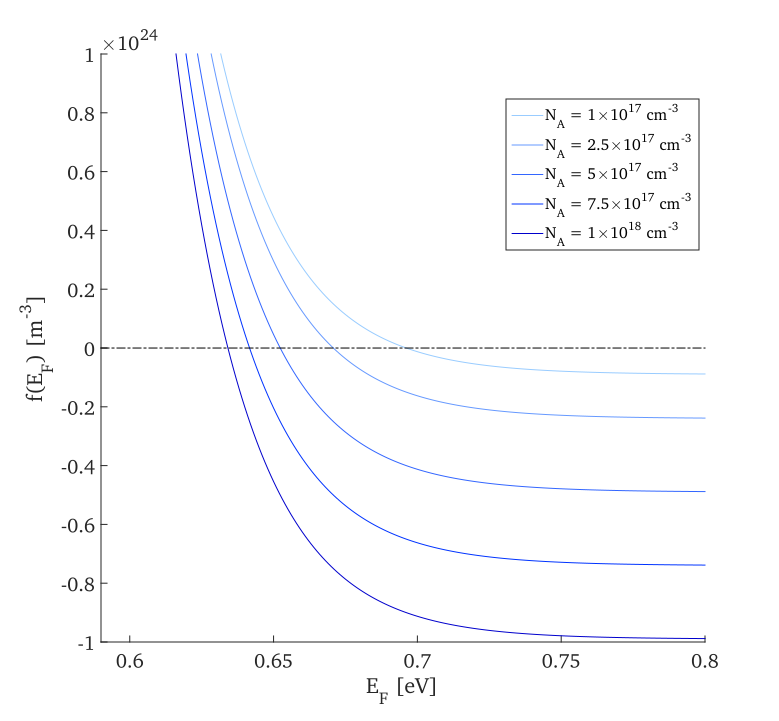
\includegraphics[scale=0.6]{N_A.pdf}
\caption{Computed values of LHS in equation \ref{eq:neutrality2}, plotted against the Fermi level. The three graphs show acceptor concentrations of $10^{17}$, $10^{18}$ and $10^{19}$ cm$^{-3}$. 
\label{fig:N_A}}
\end{center}
\end{figure}

Most of the B-doped samples showed no luminescence at all. One possible explanation for this is that the acceptor level is of non-radiative character. It is to be expected that boron, which is a deep level impurity, is of non-radiative character, and recombines in a way which does not emit a photon, such as by the Shockley-Reed-Hall process \cite{Hall1952},\cite{Shockley1952}. There have however been reports of luminescence from B-doping levels in 3C-SiC, for example by Kubawara  et al. \cite{Company1976}. This means that the fact that the B-level may be to some extent non-radiative does not entirely explain why most of the doped samples measured show no luminescence. 

Another explanation of the PL-spectra from the doped samples is that the boron doped samples are of poor crystal quality. As shown in figure \ref{fig:B_doped_micrographs1} the doped samples contain many defects. It may be that the many defects form non-radiative levels in the band gap, which compete with the boron level. This would explain why the results do not conform to those reported in literature. 

Figure \ref{fig:pl_spectrum2} shows the PL-spectrum from the only B-doped sample showing luminescence, sample D9. In this spectrum we see a peak at around 6000 Å, which corresponds to an aluminium impurity level. This means that the sample contains aluminium, which is a shallow acceptor. As it is a shallow impurity, it will be able to capture carriers more easily compared to the deep level boron impurity. It is likely that more carriers are captured in the Al-level, which decreases the number of exciton recombinations from the B-level. This may be another explanation of why no boron related lines can be seen. From this spectrum it can also be seen that there is luminescence from the hexagonal inclusions in this sample (inclusions are shown in figure \ref{fig:BGe20_micrograph} (c)). The luminescence is from the B-CB transition. It is likely that both polytypes in the same sample have similar impurity concentrations for both B and Al. This is not consistent with the hypothesis that B-Al competition is responsible for the lack of B-lines in the 3C-SiC spectra. 














































\label{sec:discussion}

%-*- mode: LaTeX; -*-

\chapter{Conclusion}
Initially the idea was to investigate how C- and Si-face grown seeds differed in growth of B-doped samples. I was not able to reproducibly grow C-face seeds which were completely cubic. Investigating the seed growth I was able to show that however the temperature conditions were changed, 3C-SiC could not grow to cover the whole growth area on C-face substrates, while on the Si-face it was possible to reproducibly do so. The reason for this is not fully understood, but the reason may be the difference inherent in the surface of C-face and Si-face 4H-SiC, such as the surface energy of the surfaces. It may also be that the steps from the off-axis cut are different on C- and Si-faces, or contributed to the different form of the spirals. 

I have shown through optical microscopy that high B-doping leads to deteriorating surface quality of the sample. For most samples the surface quality worsened with increasing B-doping concentration of the source material. From optical microscopy and absorption measurements I have shown that it is possible to grow 3C-SiC material doped with boron using the sublimation growth technique described in this thesis. The absorption measurements indicate the boron to conduction band transition, but not the valence band to boron transition. The lack of the latter is thought to be due to the position of the Fermi level near or above the boron level in the band gap. 

I have shown using LTPL-spectroscopy that the boron levels in 3C-SiC grown in this work show no luminescence related to boron. The reason for this may be a combination of the deep level nature of the boron impurity with the poor crystal quality containing non-radiative defects. These PL-measurements further show inclusions of aluminium in the samples, which may form a competing relationship with the boron in carrier capture, further limiting the possibilities of luminescence. 
\label{sec:conclusion}

%-*- mode: LaTeX; -*-

\chapter{Future work}
In this chapter I will write some of my thought of what is to be done in the future concerning these topics. 
\label{sec:future}

%\include{introduktion}
%\include{resultat}
%\include{avrundning}

%\part*{Appendix}
%\appendix
%\include{detaljer}
%\include{rtthesis-doc}


\backmatter
\small
%\bibliographystyle{plain}
\bibliography{BibTeX/Cite-General,BibTeX/Cite-Growth,BibTeX/Cite-PL,BibTeX/Cite-Solar,BibTeX/Cite-Watersplitting}
\printindex


\end{document}




